Biologically aging can be broadly characterized as "the time-dependent functional decline that affects most living organisms" \cite{López-Otín2013}. It can be observed in the reorganization of multiple interacting physiological systems operating at different spatial and temporal scales \cite{Mooney2016}. The underlying patterns of reorganization within and between these systems are highly individual, as they are subject to internal (e.g., genetic, cellular, molecular) as well as external (e.g., environmental, and lifestyle) influences \cite{Smith2020, Mooney2016, Cohen2022}. At the same time, however, overarching, generalizable patterns can be identified \cite{Salthouse2019}. The most recognizable consequences of aging are alterations in cognitive, sensory, and motor abilities that challenge the daily lives of older adults \cite{Li2002}. However, not all abilities are equally affected by declines and the alterations are highly individual. While sensory, motor abilities and cognitive abilities, such as memory and processing speed, are described as generally declining, abilities in the context of acquired knowledge, such as verbal abilities, tend to be stable or even improve with age \cite{Park2009}. Understanding brain reorganization is of particular interest because of its interrelation with behavioral alterations.

\subsection{Age related reorganization of the brain}
\label{theory:aging:brain}
Reorganization in the structure of the brain include, among others, atrophy of the gray and white matter as well as enlargement of cerebral ventricles \cite{Fjell2010}. The efficiency of neuromodulation declines mainly driven by the loss of dopaminergic receptors indicative of a reorganization of neurotransmitter systems \cite{Li2001}. Besides this, the study of the functional properties of the brain and their relationship to behavioural changes is of great interest. In neuroimaging studies, both under-activation and over-activation of brain areas have been reported in older adults compared to younger adults during performance in various tasks with sensory, cognitive as well as motor demands \cite{Reuter-Lorenz2010, Sala-Llonch2015}. In terms of activation dynamics, brain activity in response to a stimulus is often slower or delayed. Moreover, the frequency distribution of neural oscillatory activity changes with respect to a slowing of the main rhythms and altered temporal dynamics which is interpreted as changes in neural communication \cite{Courtney2021}.\\ 
By emphasising neural communication and information flow, rather than viewing the brain as functionally separate, it can be conceptualised as a complex system whose functional units, i.e. neurons, areas and subsystems, are interconnected both structurally and functionally \cite{Friston2011,Deery2023}. In this concept, functional connectivity reflects coherent patterns of activation within and between these units. Several distinct but interconnected functional networks were identified. The dynamic interplay between and within these networks is characterized by segregation and integration at different levels, characterizing the flow of information in the brain \cite{Sporns2013}. Older adults information flow tend be less efficient and is characterized by lower within network connectivity and higher between network connectivity associated with a less segregated, less modular and more integrated brain network organization \cite{Sala-Llonch2015,Deery2023, Betzel2014}. However, studies on sensorimotor and visual networks seem to be very heterogeneous, which could indicate very individual reorganization patterns \cite{Deery2023}.

\subsubsection{Dedifferentiation}
\label{theory:aging:dedif}
Age related activation patterns and functional network reorganization, can be attributed to dedifferentiation \cite{Grady2012}. Dedifferentiation refers to the loss of neural specialization or reduced distinctiveness of neural responses resulting in a diffuse, non specific recruitment of brain resources \cite{Koen2019}. Historically, the term originates from behavioral research in which an increased correlation of performance between sensory and cognitive and sensorimotor domains was reported in older adults was reported \cite{Baltes1997,Li2002}. In order to explain this behavioral dedifferentiation Li and colleagues \cite{Li2001, Li2002} provided a computational model. According to this model, deficient neurotransmitter modulation observed in older adults may affect the responsiveness of cortical neurons, leading to higher levels of neuronal noise and ultimately to less differentiated, more diffuse neuronal activation patterns in response to different stimuli \cite{Li2001,Li2002}. In several computational simulations, the authors demonstrated that the proposed model can explain not only behavioral co-variation, but also several other phenomena, such as the decrease in average behavioural performance or the increase in behavioral intra- and inter-person variability \cite{Li2000,Li2002}. In addition, the proposition of a less distinctive, less specific neuronal activation in response to stimuli could be confirmed in neuroimaging studies showing that the neural responses to various visual, cognitive and motor stimuli are less specific in older compared to young adults \cite{Tucker2019, Koen2019,Carb2011}. Recently the reorganization of functional networks as described above, i.e. less segmented and modular, and less specialised organization in older adults was framed in terms of dedifferentiation \cite{Deery2023, Koen2019, Sala-Llonch2015}.\\
\begin{figure}[h]
\label{fig:dedifferentiation}
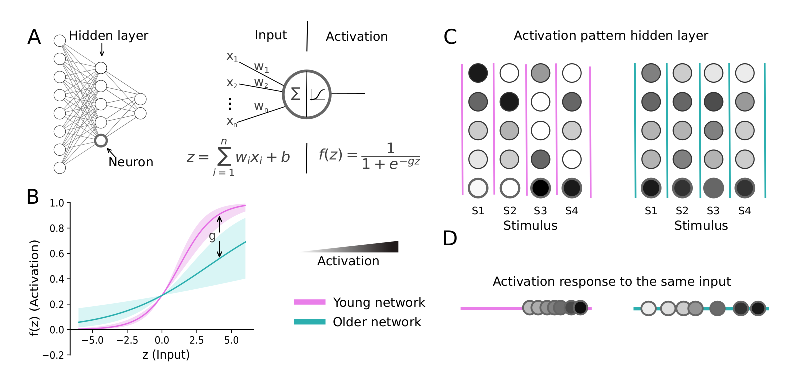
\includegraphics[width=\textwidth]{dedifferentiation.eps}
\caption{Computational model proposed by \cite{Li2000,Li2002}. The authors used a feedforward backpropagation neural network model with logistic activation function $f(z)$ and simulated altered neuromodulation by varying the gain parameter $g$ in $f(z)$. Deficient neuromodulation and responisveness due to aging is simulated by lower $g$ values (A). Simulations show that the activation pattern of simulated neurons differs less for different stimuli (B) and the activation of single neurons is more variable for multiple stimulations with the same stimulus (C).}
\end{figure}


\citeauthor{Fornito2015}\cite{Fornito2015} describe dedifferentiation as a fundamental maladaptive mechanism of brain networks that requires compensation. This is consistent with the argument that dedifferentiation and compensation are complementary mechanisms \cite{Reuter-Lorenz2010}. However, dedifferentiation could also itself represent a compensatory response, in that the brain attempts to maintain function in the face of deterioration \cite{Stern2009}. By definition compensation refers to the ability to recruit additional brain resources to compensate for decline and functional loss in order to maintain cognitive or behavioural functioning \cite{Reuter-Lorenz2010, Grady2012}. Here, the \gls{crunch} hypothesizes that compensatory activity changes as a function of task demands. Moreover, compensation often occurs in a specific pattern of under-activation of posterior areas and prefrontal over-activation, known as \gls{pasa} \cite{Davis2007}. Another often reported pattern is the more bilateral recruitment and loss of hemispheric specialisation, known as \gls{harold} \cite{Cabeza2002}.

\subsubsection{Reserve}
\label{theory:aging:reserve}
It is important to note that age related alterations of the brain and behavior are highly individual and dynamic \cite{Smith2020,Koen2019,Douw2014}. In this context, the concept of reserve was defined as the accumulated capacity of neural resources over the lifespan that can withstand decline or pathology \cite{Cabeza2018, Stern2009}. Although the concept was originally based on observations that the degree of pathological changes in the brain do not necessarily mean clinical manifestation, it has also been applied to explain individuality of non-pathological aging \cite{Esiri2001,Cabeza2018,Stern2009}.\\
Reserve can be both anatomically quantifiable, which is referred to as brain reserve, and more functional in nature, which is referred to as cognitive reserve \cite{Stern2009}. At the functional level, compensatory activation as well as more efficient utilisation (less activation of neural resources), increased capacity (increased availability of neural resources) of brain networks were described as key mechanisms of cognitive reserve \cite{Stern2004,Stern2009}. However, brain and cognitive reserve influence each other and \citeauthor{Cabeza2018} \cite{Cabeza2018} argue against a strict separation of brain reserve and cognitive reserve.\\
One aspect that explicitly determines the definition of reserve is the lifelong ability of the brain to adapt its structure and function to internal and external requirements. It is known from the animal model that environments rich in cognitive, social, as well as sensory and motor stimuli, contribute to positive plastic changes \cite{Fabel2009}. As a result, reserve is influenced by an interplay between genetic and environmental factors including lifestyle factors \cite{Cabeza2018}. Important factors for increasing reserve have been identified in education, occupation as well as physical activity, with cognitive training, physical fitness, and professional expertise having a considerable impact on the brain's functional organization \cite{vieluf2018age,VOSS2016113,Soldan2021}.\\
This is further supported by other complementary concepts such as the maintenance or the \gls{stac} models. The concept of maintenance emphasizes the ability to repair. \Gls{stac} postulates that lifelong positive and negative plasticity define a framework that enables compensation and shapes the individual trajectory of aging \cite{Reuter-Lorenz2014}. 

\subsection{Studying brain aging by electroencephalography}
The complex interplay of the aforementioned factors leading to the dynamics of age related reorganization of the brain is highly complex. Understanding these dynamics in terms of individual trajectories and overarching patterns is a prerequisite to differentiate healthy from pathological changes and to develop and verify treatments as well as targeted interventions. This requires uncomplicated, easy-to-use, and cost-effective methods and novel analyses to quantify changes in brain organization. Several noninvasive methods are available to study the brains' structure and function. \Gls{mri} is the most widely used method in science to image the structure or, using \gls{fmri}, the function of the brain, which is the dominant method in the study of the functional reorganization described in the previous section \cite{Reuter-Lorenz2010}. However, this method is very costly and requires expertise that is not widely available. As a result, its use in the public health system is mostly limited to cases with a clear indication, so that early detection of unfavourable aging trajectories is rather difficult. In addition, limited availability substantially restricts the development of preventive and rehabilitative interventions and therapies and excludes areas and sites with low levels of equipment and expertise. Here, \gls{eeg} could represent a real added value, since it is characterized by a simple use, mobility, and relative cost effectiveness. Although it has a lower spatial resolution than \gls{mri} based methods, \gls{eeg} measures neuronal activity directly with high temporal resolution which allows for the detection of age-related changes in the temporal dynamics of brain activity and networks, which could be of special interest to understand age related changes of the brain and their relation to behavior \cite{Courtney2021}.

\begin{tcolorbox}[breakable, enhanced]
    \subsubsection{Excursus: A brief overview on electroencephalography}
    \Gls{eeg} measures time varying electrical fields on the surface of the head by using several sensors placed in a standardized position \cite{Jackson2014}. The measured signals reflect synchronously active populations of neurons. Electrical activity can only accumulate and be detected on the surface of the head if spatially similar neurons, aligned perpendicular to the surface, are synchronously activated. Based on the conductive properties of the brain the signal can travel through the different layers to the surface due to volume conduction. For this reason, and due to the orientation of the neural cell assemblies, the signal in each sensor reflects a summed signal of different neuron patches. The signals expressions are in the range of a few microvolts and is much lower than other biological and non-biological electrical generators, e.g. muscular activity or line noise, so that the EEG signal is often affected by a low signal-to-noise ratio.\\
    One of the most striking signal characteristics of the EEG is the rhythmic fluctuations in voltage that define the signal and are summarized under the term oscillation. It is common that the EEG signal is analyzed based on the frequency composition of oscillatory activity in loosely defined frequency ranges, i.e., $\delta$ ($<$4 Hz), $\theta$ (4-8 Hz), $\alpha$ (8-12 Hz), $\beta$ (12-30 Hz) and $\gamma$ ($>$30 Hz), which have been demonstrated to be related to perceptual, cognitive, motor and emotional processes \cite{CohenX2017}. Furthermore, the analysis of frequency-dependent synchrony or functional connectivity in terms of a statistical dependence of the signals, e.g. by coherence or the phase synchrony of the signal, can provide information about the network characteristics of the brain \cite{Siegel2012}. Finally, the analysis of event-related activation, so called \glspl{erp}, can furthermore provide information on the direct processing of stimuli. This involves time-locking the EEG data to the onset of a specific stimulus and averaging the EEG signal across multiple trials to extract a reliable signal that is related to the processing of the stimulus.
\end{tcolorbox}

\subsubsection{Electroencephalographic signatures of age-related reorganization}
Age related changes in these \gls{eeg} characteristics have been extensively studied. Specifically it has been reported that aging is associated with changes in the frequency composition of the EEG signal, regardless of any specific task involvement. These changes include a decrease in amplitude within the $\alpha$ frequency band, a shift in the $\alpha$ peak frequency towards lower frequencies, an increase in amplitude within the $\beta$ frequency band, and varying results regarding changes in the amplitude of the theta and delta bands \cite{ROSSINI2007375, Ishii2017, Courtney2021}. Moreover, age related changes have also been reported in terms of reduced \gls{eeg} synchrony and a more random less segregated organization of \gls{eeg} derived network topology \cite{Smit2012, Samogin2022}.\\
\Gls{eeg} changes in relation to tasks are highly dependent on the task context or domain studied. For example, unilateral motor tasks may display lower frequency specificity and more bilateral spatial expression of $\alpha$ and $\beta$ frequency power modulations, while attention tasks may demonstrate enhanced frontal network involvement as well as power in the $\theta$ frequency band \cite{Hong2016,Quandt2016}. In addition, the neural response to stimuli may exhibit a temporal slowing and altered spatial expression. This can be seen, for example, in a delay of early \gls{erp} components in visual attention tasks and more frontal expression of later \gls{erp} components and \cite{LI2013477, Reuter2017}.
Often these changes are discussed in relation to the mechanisms of dedifferentiation and compensation described above which have been show to be modulated by lifetime experience such as occupational expertise \cite{vieluf2018age} or physical fitness \cite{Douw2014}.\\ 
However, the relationship between \gls{eeg} parameters and these mechanisms often seems to be ambiguous. As such, other \gls{eeg} findings may point in the opposite direction than described above. \citeauthor{HUBNER2018104}\cite{HUBNER2018104} for instance found no age effects in central lateralization in the $\beta$ frequency band in a complex fine motor control task, which again highlights the dependency to the task context considered. Age-related changes in decreased \gls{erp} latency as well as lower or increased functional connectivity of the examined networks depending on the task context are also reported \cite{Courtney2021}. Moreover, the interpretation of dedifferentiation is often based on \gls{fmri} findings that report over-activation and loss of segregation of brain networks. However, the relationship between frequency-specific \gls{eeg} and \gls{fmri} findings acting on completely different spatial and time scales as well as measurement principles is not clear. \citeauthor{Koen2019} \cite{Koen2019} further points out that over-activation should be interpreted cautiously and does not necessarily imply loss of neural specificity, as predicted in the original model of \citeauthor{Li2000}\cite{Li2000}. He therefore proposes to operationalize dedifferentiation clearly in terms of the selectivity of the neural response between two or more task modulations. While in this operationalization the evidence regarding dedifferentiation in \gls{fmri} studies is quite clear, this has not been explored in \gls{eeg} studies so far \cite{Koen2019}.\\
\\
Altogether the \gls{eeg} represents an easy-to-use, low-cost alternative to \gls{fmri} and provides additional insight into age-related changes. However, the link to age-related changes reported consistently in the \gls{fmri} such as dedifferentiation is often difficult and not entirely clear or unknown. Furthermore, \gls{eeg} signals are temporally and spatially highly dimensional and have a low signal-to-noise ratio, which makes the detection and visualization of age related brain reorganization and their dynamics difficult and requires advanced signal analysis methods. Advanced methods such as methods from the field of machine learning could be of special interest in this context.